\documentclass[tikz]{standalone}
\usepackage{pgfplots}
\usepgfplotslibrary{groupplots}
\pgfplotsset{compat=1.18}
\definecolor{utnblue}{RGB}{0, 102, 204}

\begin{document}
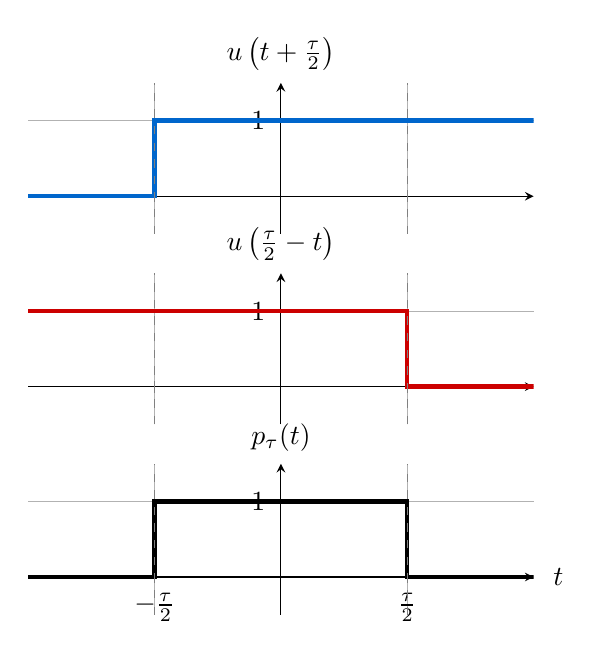
\begin{tikzpicture}
    \begin{groupplot}[
        group style={
            group size=1 by 3,
            vertical sep=0.5cm,
        },
        width=8cm,
        height=3.5cm,
        axis x line=middle,
        axis y line=center,
        xmin=-4, xmax=4,
        ymin=-0.5, ymax=1.5,
        xtick={-2, 2},
        xticklabels={$-\frac{\tau}{2}$, $\frac{\tau}{2}$},
        ytick={1},
        grid=both,
        grid style={line width=.1pt, draw=gray!40},
        major grid style={line width=.2pt,draw=gray!60},
        samples=100,
        enlarge x limits=false,
        every axis plot/.append style={ultra thick},
        every axis x label/.append style={at={(ticklabel* cs:1.02)}, anchor=west},
        every axis y label/.append style={at={(rel axis cs:0.5, 1.02)}, anchor=south, rotate=0}
    ]
    
    % Panel 1: u(t + \tau/2)
    \nextgroupplot[ylabel={$u\left(t + \frac{\tau}{2}\right)$}, xticklabels={,,}]
    \addplot[color=utnblue] coordinates {(-5,0) (-2,0) (-2,1) (5,1)};
    \draw[dashed, gray] (-2,-0.5) -- (-2,1.5);
    \draw[dashed, gray] (2,-0.5) -- (2,1.5);

    % Panel 2: u(\tau/2 - t)
    \nextgroupplot[ylabel={$u\left(\frac{\tau}{2} - t\right)$}, xticklabels={,,}]
    \addplot[color=red!80!black] coordinates {(-5,1) (2,1) (2,0) (5,0)};
    \draw[dashed, gray] (-2,-0.5) -- (-2,1.5);
    \draw[dashed, gray] (2,-0.5) -- (2,1.5);

    % Panel 3: Product
    \nextgroupplot[ylabel={$p_\tau(t)$}, xlabel={$t$}]
    \addplot[color=black] coordinates {(-5,0) (-2,0) (-2,1) (2,1) (2,0) (5,0)};
    \draw[dashed, gray] (-2,-0.5) -- (-2,1.5);
    \draw[dashed, gray] (2,-0.5) -- (2,1.5);
    
    \end{groupplot}
\end{tikzpicture}
\end{document}
